\documentclass[journal]{./IEEE/IEEEtran}
\usepackage{amsmath,apacite,graphicx,microtype,tikz,xurl, pgfplots, listings, xcolor}

\pgfplotsset{compat=1.18}
\lstset{
    basicstyle=\ttfamily\footnotesize,
    breaklines=true,
    frame=single,
    backgroundcolor=\color{gray!5},
    columns=fullflexible,
    keepspaces=true,
    showstringspaces=false
}

\newcommand{\SPTITLE}{Enhancing Cereal Crops Phenotypic Trait Searchability and Parental Line Selection Using Retrieval-Augmented Semantic Search}
\newcommand{\ADVISEE}{Zach Dwayne M. Glindro}
\newcommand{\ADVISER}{Mylah Rystie U. Anacleto}

\newcommand{\BSCS}{Bachelor of Science in Computer Science}
\newcommand{\ICS}{Institute of Computer Science}
\newcommand{\UPLB}{University of the Philippines Los Ba\~{n}os}
\newcommand{\REMARK}{\thanks{Presented to the Faculty of the \ICS, \UPLB\
                             in partial fulfillment of the requirements
                             for the Degree of \BSCS}}
        
\markboth{CMSC 190 Special Problem, \ICS}{}
\title{\SPTITLE}
\author{
  \ADVISEE,~%
  \ADVISER,~%
  Mark Anthony~L.~Parducho,~%
  Ayn Kristina~M.~Beltran,~%
  and~Maria Alma~B.~Sanchez%
  \REMARK
}
% \pubid{\copyright~2006~ICS \UPLB}

%%%%%%%%%%%%%%%%%%%%%%%%%%%%%%%%%%%%%%%%%%%%%%%%%%%%%%%%%%%%%%%%%%%%%%%%%%

\begin{document}

% TITLE
\maketitle

% ABSTRACT
\begin{abstract}
Plant breeding research currently relies on the manual analysis of extensive phenotypic trait data within spreadsheets, a method fundamentally limited by rigid, keyword-based search mechanisms. To address this, a Retrieval-Augmented Generation (RAG) system was designed and implemented, leveraging dense vector embeddings and a two-stage hybrid retrieval pipeline to facilitate natural language querying of phenotypic databases. This system was evaluated against a standard BM25 keyword baseline using 20 complex agricultural queries and standard information retrieval metrics. Quantitative results demonstrate that the hybrid approach outperforms lexical search in Precision@k, successfully navigating nuanced agricultural terminology where traditional keyword matching fails. Usability trials with research personnel further compared the AI-driven interface against established Microsoft Excel-based workflows, revealing a distinct reliability gap between system performance and user workflow expectations. Findings indicate researchers prioritize the deterministic precision and predictable accuracy of spreadsheet filters over the probabilistic "fuzziness" of semantic retrieval. Ultimately, this research concludes that while semantic search offers a scalable solution for data discovery, future agricultural information systems must adopt a filter-first co-pilot paradigm—leveraging AI to generate structured database filters before performing semantic retrieval—to ensure the exactitude required for scientific breeding decisions.
\end{abstract}

% INDEX TERMS
\begin{keywords}
retrieval-augmented generation, semantic search, plant breeding, phenotypic traits, large language models, vector database, natural language processing
\end{keywords}

% INTRODUCTION
\section{Introduction}

\subsection{Background of the Study}
In plant breeding, the goal is to develop new and improved crop varieties by selecting ``parental lines'' that possess desirable characteristics. To make these selections, researchers rely on large amounts of phenotypic trait data, which are often recorded and managed using general-purpose spreadsheets like Microsoft Excel or Google Sheets. This common practice requires researchers to manually search through rows and columns of data to find the information they need.

The main problem with using spreadsheets is their reliance on simple keyword-based search, such as using the "Find" or "Search" function. This type of search is literal; it only finds data that exactly matches the typed words. This approach is rooted in older information retrieval methods that represent text as a collection of keywords, using techniques like Term Frequency-Inverse Document Frequency (TF-IDF) to determine relevance~\cite{zhao_dense_2024}. This creates a ``semantic gap'', where if a researcher searches for ``lodging resistance,'' the system will not find entries that use synonyms or related phrases like ``strong stems'' or ``resists stem breakage.'' This forces researchers to remember the exact terminology used during data entry, which can vary among different personnel and over time. As a result, search results are often incomplete, and valuable parental lines can be missed, making the data search process inefficient~\cite{garcia_improving_2025}.

To overcome these limitations, modern information retrieval has shifted towards semantic search. Semantic search focuses on understanding the meaning behind a query rather than just matching keywords. This approach is made possible by pre-trained language models (PLMs), which can transform text into dense vector representations called "embeddings"~\cite{mandikal_sparse_2024,zhao_dense_2024}. Models like Sentence-BERT are specifically designed to create embeddings where similar concepts are located close to each other in vector space, allowing for effective similarity comparisons using metrics like cosine similarity~\cite{reimers_sentence-bert_2019}. This turns the search problem into a nearest neighbor search, which can be efficiently handled by specialized vector databases~\cite{zhao_chat2data_2024}.

This study applies these techniques using a framework called Retrieval-Augmented Generation (RAG). A RAG system has two main parts: a "retriever" that uses semantic search to find the most relevant pieces of information from a knowledge base, and a "generator," which is a large language model (LLM) that takes this retrieved information as context to provide a clear and accurate answer~\cite{lewis_retrieval-augmented_2021}. This approach has been successful in other specialized fields, such as agriculture and biomedicine, because it grounds the LLM's responses in factual data, which helps to avoid errors and "hallucinations"~\cite{balaguer_rag_2024,garcia_improving_2025,hier_simplified_2025, soong_improving_2024}. By building a RAG-based semantic search system, this study aimed provide plant breeders with a more intuitive and effective way to analyze phenotypic trait data, ultimately improving the efficiency of parental line selection.

\subsection{Statement of the Problem}
Traditional methods for analyzing phenotypic trait data in plant breeding often rely on general-purpose spreadsheets like Microsoft Excel and Google Sheets. The primary mechanism for data retrieval in these applications is keyword-based lexical search, which is fundamentally limited by its reliance on exact string matching. This rigidity creates a barrier to data , placing a burden on the user's recall of specific terminology and data entry standards, which can vary between researchers and over time. Consequently, this leads to incomplete search results, risking the omission of parental lines from consideration.

Recent advancements in natural language processing, particularly in dense embeddings and retrieval-augmented generation (RAG) offer a solution to this challenge. This study aimed to bridge this semantic gap by designing and evaluating a system that leverages these technologies. By doing so, the system empowers researchers to find data based on conceptual meaning, thereby improving the efficiency of parental line selection.

\subsection{Significance of the Study}
This study aimed to demonstrate a practical framework to transition from keyword-based data retrieval in spreadsheets to a flexible semantic search system for phenotypic trait data. This shift alleviates the burden on researchers to recall exact terminology and adhere to strict data standards, which hinder effective data . The system allows users with varying levels of technical expertise, from researchers to lab technicians, to query the database using natural, descriptive language and receive conceptually relevant results. By providing a practical case study on applying retrieval-augmented generation and large language models to a specialized scientific domain, this study aimed to improve the efficiency of parental line selection and offer a model for integrating semantic search into other research fields grappling with similar data accessibility challenges.

\subsection{Objectives of the Study}
The general objective of the study is to design, implement, and evaluate a retrieval-augmented semantic search system to improve the efficiency and accuracy of phenotypic trait searchability. The specific objectives are the following:

\begin{enumerate}
    \item To develop a Retrieval-Augmented Generation (RAG) pipeline using a sentence embedding model and a vector database for indexing and searching phenotypic trait descriptions
    \item To integrate the semantic search pipeline into a web application to provide a natural language interface for researchers
    \item To evaluate the performance of the semantic search system against a traditional keyword-based search baseline, using standard information retrieval metrics: Precision@k, Recall@k, and Mean Average Precision (MAP); and
    \item To assess the web application's effectiveness and usability in facilitating parental line selection.
\end{enumerate}

\subsection{Scope and Limitations of the Study}
This study focuses on the design, implementation, and evaluation of a web application that leverages a retrieval-augmented generation (RAG) pipeline for semantic search on phenotypic trait data. The system is specifically tailored to the Cereal Crops Section at the Institute of Plant Breeding to facilitate more efficient parental line selection. The study will not address challenges related to large-scale, enterprise-level performance, such as handling high user concurrency. The application is designed for a small group of researchers in a self-hosted environment. Furthermore, the system's development and evaluation will be confined to the provided trait data, and its applicability to other crop types will not be formally assessed.

\section{Review of Related Literature}

\subsection{Lexical and Semantic Search}
Information Retrieval (IR) has been characterized by a fundamental progression from matching literal words to understanding conceptual meaning. Early IR systems are built upon the principle of lexical search, where documents and queries are represented as high-dimensional, sparse vectors under the "bag-of-words" assumption~\cite{zhao_dense_2024}. In this vector-space model, each dimension corresponds to a specific term in the vocabulary, and the relevance of a document is determined by the presence and frequency of query terms. Techniques such as Term Frequency-Inverse Document Frequency (TF-IDF) and the probabilistic BM25 algorithm became the standard for weighting the importance of terms and scoring documents~\cite{zhao_dense_2024}. The primary strength of this sparse-vector approach is in its efficiency and precision for queries that depend on exact keyword matching. However, it fails to retrieve semantically relevant documents that use synonyms, related concepts, or descriptive language instead of the exact query terms.

To address the limitations of lexical search, a shift toward semantic search has occurred, driven by the capabilities of pre-trained language models (PLMs). This approach moves beyond keyword matching to interpret the conceptual meaning behind a user's query. PLMs like BERT and its specialized derivatives for scientific text, such as SciBERT and SPECTER2, are now used to encode the contextual meaning of text into low-dimensional, dense vectors called embeddings~\cite{mandikal_sparse_2024}. In this paradigm, both queries and documents are mapped into a shared latent semantic space. Relevance is then measured not by keyword overlap but by the proximity of their respective vectors, typically calculated using cosine similarity or inner product~\cite{zhao_dense_2024}. This process transforms the retrieval task into a nearest neighbor search problem, which can be accelerated through specialized dense vector databases that use indexing techniques~\cite{monir_vectorsearch_2024,zhao_chat2data_2024}. This dense retrieval mechanism forms the core of modern systems like Retrieval-Augmented Generation (RAG), where a retriever, such as the Dense Passage Retriever (DPR), is trained to fetch relevant documents to provide as context for a generator model, grounding its responses in factual, external knowledge~\cite{lewis_retrieval-augmented_2021}.

While dense retrieval models excel at understanding semantic nuance, recent studies indicate that they are not a replacement for sparse methods. Dense models can sometimes struggle with queries that contain rare keywords, specific identifiers, or technical terms where the precision of lexical matching is prioritized~\cite{sawarkar_blended_2024}. This has led to the emergence of hybrid or "blended" retrieval as the new state-of-the-art. Mandikal \& Mooney~\cite{mandikal_sparse_2024} demonstrated on a scientific document benchmark that a dense retriever performed only comparably to a traditional sparse model, but a simple hybrid approach that combined the scores of both significantly outperformed either method in isolation. More sophisticated systems, termed "Blended RAG," take this further by using multiple indices, such as sparse BM25, dense vector, and sparse encoder indices, along with hybrid query strategies to synthesize the strengths of each~\cite{sawarkar_blended_2024}. This consensus suggests that combining the keyword-matching precision of sparse retrieval with the conceptual understanding of dense retrieval provides a more robust and accurate solution, which is crucial for industry-specific applications like agriculture where both general and specific terminology must be handled effectively~\cite{balaguer_rag_2024}.

\subsection{Dense Embeddings and Pre-Trained Language Models}
The development of Pre-Trained Language Models (PLMs), founded on the Transformer architecture, has been central to the shift toward semantic search. These models follow a "pretrain, then fine-tune" paradigm, learning to encode the contextual meaning of text into low-dimensional, dense vectors, or embeddings~\cite{zhao_dense_2024}. However, standard PLMs like BERT were not originally designed for semantic similarity search. Because they require both sentences to be fed into the network simultaneously, finding the most similar pair in a large collection involves a massive computational overhead, making them impractical for first-stage retrieval~\cite{reimers_sentence-bert_2019}. To solve this, two main architectures have emerged: the accurate but computationally expensive cross-encoder, which processes query-document pairs together for re-ranking, and the efficient bi-encoder, which creates independent embeddings for queries and documents, making it ideal for initial retrieval~\cite{zhao_dense_2024}. The Sentence-BERT model was a key innovation in this area, using a siamese bi-encoder structure to generate semantically meaningful embeddings that could be efficiently compared using cosine similarity, making PLMs practical for large-scale semantic search~\cite{reimers_sentence-bert_2019}.

While powerful, general-purpose PLMs often lack the specialized vocabulary and domain knowledge required for technical fields. This has led to the development of models that undergo pre-training on domain-specific corpora. In the scientific and clinical domains, models such as BioBERT, ClinicalBERT, and PhenoBCBERT have been fine-tuned on biomedical literature and clinical notes to improve performance on tasks like phenotype recognition~\cite{yang_enhancing_2024}. Similarly, models like SciBERT and SPECTER2 are adapted for scientific literature to better represent the nuances of research documents~\cite{mandikal_sparse_2024}. A more fundamental challenge arises when applying PLMs to structured data. Early models like TaBERT addressed this by learning joint representations for natural language and tables, linearizing rows and using relevant "context snapshots" to encode the table's structure~\cite{yin_tabert_2020}. This principle has evolved in modern text-to-SQL systems, which use RAG to provide database schema and diverse examples as context, enabling LLMs to generate accurate queries from natural language questions, complete with error-correction loops for validation~\cite{thorpe_dubo-sql_2024}.

A more recent paradigm shifts the focus from resource-intensive pre-training on raw data to taking advantage of the vast knowledge contained within scientific literature via large, general-purpose Large Language Models (LLMs) like the GPT series. The GenePT model exemplifies this approach by generating gene and cell embeddings directly from their textual descriptions in curated databases like NCBI, using a powerful off-the-shelf embedding model from ChatGPT~\cite{chen_genept_2023}. This method composes representations for complex entities, such as a single cell, by either creating a weighted average of the embeddings of its constituent genes or by forming a sentence-like sequence of gene names ordered by expression level to be embedded as a whole. This approach offers an effective path for creating biological foundation models, as it bypasses the need for extensive data curation and pre-training while capturing a high-level, human-curated knowledge source that often results in comparable or superior performance on domain-specific tasks~\cite{chen_genept_2023}.

Despite the high accuracy of transformer-based bi-encoders, their reliance on the self-attention mechanism introduces significant latency, particularly on CPU-based systems or in environments with limited hardware resources. To bridge the gap between performance and efficiency, a recent paradigm shift involves the distillation of large transformer models into high-performance "static" embeddings. Using frameworks like \textit{model2vec}, the high-dimensional knowledge of models like \textit{mxbai-embed-large-v1} can be compressed into a fixed vocabulary lookup table through techniques like weight-averaging and k-means clustering of token embeddings~\cite{minishlab2024model2vec}. 

Models such as \texttt{potion-mxbai-micro} represent the extreme of this efficiency, reducing model size to under one megabyte while maintaining a significant portion of the original model's semantic capabilities. Because these models eliminate the need for a heavy neural network pass during inference—relying instead on pure NumPy-based lookups—they can achieve up to 80-fold increases in speed on standard consumer CPUs compared to traditional bi-encoders. This makes them uniquely suited for real-time agricultural search applications where rapid response times are prioritized over the massive parameter counts of general-purpose language models.

\subsection{Vector Databases}
Semantic search requires specific infrastructure for managing the dense vector embeddings that represent conceptual meaning. Traditional relational databases, designed for structured data and exact matching, are not suited for the high-dimensional similarity search required by these embeddings~\cite{ma_comprehensive_2025}. This has led to the emergence of vector databases (VDBs), which are purpose-built systems for the efficient storage and retrieval of large-scale vector collections~\cite{monir_vectorsearch_2024}. A core principle of VDBs is the shift from Nearest Neighbor Search (NNS), which is computationally infeasible for large datasets, to Approximate Nearest Neighbor Search (ANNS). ANNS algorithms compromise a small degree of accuracy for gains in search speed and reductions in memory usage~\cite{ma_comprehensive_2025, douze_faiss_2025}.

VDBs rely on ANNS indexing strategies that effectively prune the search space. One of the most prominent strategies is the graph-based method, exemplified by the Hierarchical Navigable Small World (HNSW) algorithm. HNSW constructs a multi-layered graph where connections are separated by distance-scale; long-range links in the upper layers allow for rapid traversal across the vector space, while short-range links in the lower layers enable precise local search, resulting in logarithmic search complexity~\cite{malkov_efficient_2020}. Another strategy is quantization, which compresses vectors to reduce their memory footprint and accelerate distance calculations. Product Quantizations (PQ) is a widely used technique that achieves this by splitting a vector into sub-vectors and encoding each one separately, enabling distance comparisons to be performed quickly in the compressed domain through either Asymmetric or Symmetric Distance Computation~\cite{douze_faiss_2025}. These techniques are often combined into hybrid architectures, such as the Inverted File system with Product Quantization (IVFPQ), which first partitions the data into clusters using a coarse quantizer and then applies PQ to the residual vectors within each cluster, narrowing the search to only the most promising partitions~\cite{ma_comprehensive_2025, douze_faiss_2025}.

The practical implementation of the ANNS algorithms is largely-driven by open-sources libraries that have become industry standards. Faiss, for instance, provides a toolkit offering a wide variety of indexing and compression methods, including PQ, IVF, and HNSW, allowing practitioners to build customized indexing pipelines~\cite{douze_faiss_2025}. The selection of an appropriate index and the tuning of its hyperparameters, such as nprobe for IVF or efConstruction for HNSW, are design decisions that depend on dataset size, memory constraints, and the desired accuracy-speed trade-off~\cite{monir_vectorsearch_2024}. Within RAG systems, VDBs serve as the foundational retrieval component. They store the embeddings of external knowledge sources and, upon receiving a query, rapidly fetch the most semantically relevant documents to provide as context for a large language model~\cite{zhao_chat2data_2024}. This grounds the model's responses in factual data and enables functionalities like real-time semantic caching, which reduces latency and the computational cost of frequent LLMS interactions~\cite{zhao_chat2data_2024}.

\subsection{NLP for Automated Phenotyping}
The need to analyze large volumes of phenotypic data is a challenge shared across scientific disciplines, from clinical medicine to agriculture. In both fields, the goal is to overcome the time-consuming nature of manual analysis by developing automated methods~\cite{garcia_improving_2025, hier_simplified_2025}. A key step in this process is mapping descriptive, human-readable trait observations to standardized, machine-readable terms within a controlled vocabulary. While the biomedical field has a well-established standard in the Human Phenotype Ontology (HPO), agriculture uses its own specific trait dictionaries and ontologies. Early NLP approaches to this task, such as the dictionary-based tools ClinPhen and Doc2HPO used in clinical settings, relied on concept recognition through lexical matching. These systems function by comparing text segments against a predefined vocabulary, but their rigidity makes them inflexible to linguistic variation like synonyms or paraphrasing and unable to interpret nuanced contexts, leading to incomplete data extraction and a high rate of false positives that require manual review~\cite{garcia_improving_2025, yang_enhancing_2024}.

The limitations of lexical matching prompted a shift toward more sophisticated models capable of contextual understanding. This began with Transformer-based models like BERT and its domain-specific variants, which offered improved performance over rule-based systems~\cite{yang_enhancing_2024}. While the application of general-purpose LLMs from the GPT series showed greater promise, a significant weakness emerged, primarily their propensity for errors and "hallucinations" when tasked with generating precise, factually correct identifiers from an ontology~\cite{garcia_improving_2025, soong_improving_2024}. This unreliability poses a major barrier to adoption in scientific research. To address this, Retrieval-Augmented Generation (RAG) has become the state-of-the-art solution. The RAG framework grounds LLM responses in a reliable, external knowledge source, in this case a database of standardized traits. A "retriever" component first finds relevant candidate terms from the ontology via semantic similarity, and these candidates are then provided as context within the LLM's prompt. This constrains the "generator" to select the most appropriate term from a factually accurate list. The success of this approach in the biomedical domain, where studies have shown RAG can boost normalization accuracy from 62\% to 85\%~\cite{hier_simplified_2025} while drastically reducing hallucinations~\cite{garcia_improving_2025}, provides a precedent for applying the same principles to agricultural trait .

\subsection{Evaluation}
Evaluating the quality of system outputs has shifted from relying on manual human evaluation to incorporating automated methods for efficiency and scalability, especially for offline evaluation where live A/B testing is impractical. A prominent approach is the "LLM-as-a-Judge" paradigm, which leverages a powerful language model like GPT-4 to act as a proxy for human evaluators~\cite{zheng_judging_2023}. This concept has been implemented in practice through automated pipelines that use carefully engineered prompts and custom metrics, such as "on-topic rate," to measure semantic relevance in search results, reporting consistency rates with human annotators of over 81\%~\cite{zheng_semantic_2024}. While this automated judgment focuses on task-specific criteria like relevance and groundedness~\cite{balaguer_rag_2024}, LLM judges have been shown to exhibit inherent biases toward position and verbosity, underscoring the role of human evaluation as the "gold standard" for assessment~\cite{zheng_judging_2023}.

Alongside qualitative judgments, system performance is quantitatively assessed through a combination of standard NLP, information retrieval (IR), and efficiency metrics. To measure the quality of generated text against reference answers, n-gram-based overlap metrics such as ROUGE, BLEU, and METEOR are commonly employed~\cite{radeva_web_2024}. Beyond lexical similarity, the conceptual closeness between generated and reference texts is measured using cosine similarity on their vector space representations. The model's predictive certainty is further evaluated using perplexity, where a lower score indicates higher confidence~\cite{radeva_web_2024}. For the retrieval component of the system, effectiveness is measured with standard IR metrics, including Precision, Recall, and F1-Score, which assess the accuracy of the search results~\cite{radeva_web_2024}. In systems that generate executable outputs, such as SQL queries, Execution Accuracy (EX) is used to verify that the output runs correctly and yields the expected results~\cite{hong_next-generation_2025}. Finally, the practical efficiency of the system is benchmarked by its speed and throughput, using metrics like total evaluation time and tokens per second~\cite{radeva_web_2024}.

% MATERIALS AND METHODS
\section{Materials and Methods}

\subsection{System Architecture}
The system was designed as a client-server web application that integrates a Retrieval-Augmented Generation (RAG) pipeline to provide semantic search capabilities over phenotypic trait data. The architecture, illustrated in Figure \ref{fig:architecture}, was composed of a frontend user interface, a backend server with a REST API, a relational database for storing original data, and a vector database for enabling semantic search.

\begin{figure}
    \centering
    \includegraphics[width=0.5\linewidth]{images/updated_system_arch.png}
    \caption{System Architecture of the RAG-based application.}
    \label{fig:architecture}
\end{figure}

The application provides two distinct interaction modes to facilitate data exploration and management:

\begin{enumerate}
\item \textbf{Conversational RAG (Chat Mode):} Located on the home page, this interface allows users to interact with the \textit{Qwen3-0.6B} LLM. The LLM acts as an autonomous agent equipped with a custom "search tool." When a user submits a natural language query, the LLM determines if a database lookup is required. If so, it invokes the tool to trigger the semantic search pipeline, synthesizes the retrieved records into a natural language summary, and presents the formatted data to the user.
\item \textbf{Direct Semantic Search (Edit Mode):} Located on the data page, this interface provides a traditional tabular view of the dataset. It allows for direct semantic querying of the vector database without LLM intervention. This mode also supports administrative tasks, including record updates and dynamic schema modifications such as adding or deleting columns via context menus.
\end{enumerate}

The user interaction flow is as follows:
\begin{itemize}
    \item A researcher inputs a natural language query into the web interface.
    \item The frontend transmits the query to the backend API.
    \item The backend server converts the query into a dense vector embedding using the \textit{potion-mxbai-micro} bi-encoder.
    \item This vector is used to perform an Approximate Nearest Neighbor (ANN) search against the ChromaDB vector database to retrieve an initial candidate set of results.
    \item The query and the candidate records are passed to the \textit{jina-reranker-v1-tiny-en} cross-encoder. This model re-scores and re-ranks the candidates to ensure the most semantically relevant rows are at the top of the list.
    \item The unique identifiers from the top re-ranked results are used to fetch the full records from the SQL database.
    \item The retrieved data is passed to the LLM for summarization.
    \item The backend returns both the generated summary and the re-ranked structured data to the frontend.
\end{itemize}

\subsection{Data Acquisition and Preprocessing}
\begin{figure*}[htbp]
\centering
\resizebox{\textwidth}{!}{
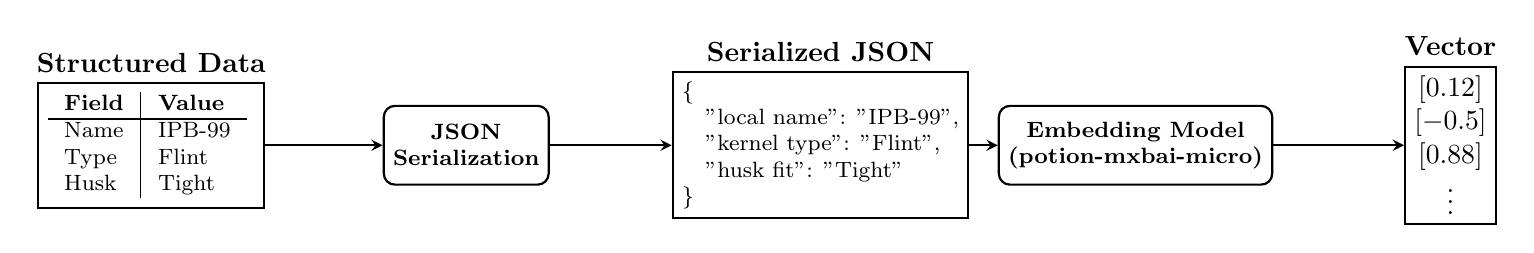
\begin{tikzpicture}[
    node distance=1.5cm,
    % Define styles for the boxes
    databox/.style={rectangle, draw=black, thick, align=left, minimum width=2.5cm, minimum height=1.5cm, font=\footnotesize},
    process/.style={rectangle, draw=black, thick, rounded corners, minimum width=2cm, minimum height=1cm, align=center, font=\footnotesize\bfseries},
    arrow/.style={->, >=stealth, thick}
]

\node (table) [databox, label=above:\textbf{Structured Data}] {
    \begin{tabular}{l|l}
    \textbf{Field} & \textbf{Value} \\ \hline
    Name & IPB-99 \\
    Type & Flint \\
    Husk & Tight \\
    \end{tabular}
};

\node (template) [process, right of=table, xshift=2.5cm] {JSON\\Serialization};

\node (text) [databox, right of=template, xshift=3.0cm, label=above:\textbf{Serialized JSON}] {
    \{ \\
    \hspace{1em}"local name": "IPB-99", \\
    \hspace{1em}"kernel type": "Flint", \\
    \hspace{1em}"husk fit": "Tight" \\
    \}
};

\node (model) [process, right of=text, xshift=2.5cm] {Embedding Model\\(potion-mxbai-micro)};

\node (vector) [rectangle, draw=black, thick, right of=model, xshift=2.5cm, align=center, label=above:\textbf{Vector}] {
    $[0.12]$ \\ $[-0.5]$ \\ $[0.88]$ \\ $\vdots$
};

\draw [arrow] (table) -- (template);
\draw [arrow] (template) -- (text);
\draw [arrow] (text) -- (model);
\draw [arrow] (model) -- (vector);

\end{tikzpicture}
}
\caption{The data preprocessing pipeline.}
\label{fig:pipeline}
\end{figure*}

The system was developed and evaluated using the original phenotypic dataset provided by the Cereal Crops Section of the Institute of Plant Breeding. This dataset comprises 3,682 unique parental line records. Each record is highly multidimensional, containing 131 distinct columns covering passport data (e.g., Region, Province, Collection Date), morphological traits (e.g., Kernel Color, Silk Color, Plant Height), and biotic/abiotic stress responses (e.g., Waterlogging, Downy Mildew, and Calcareous Soil resistance).

To prepare this high-dimensional structured data for semantic search, a preprocessing pipeline (Fig. \ref{fig:pipeline}) was implemented to transform each row into a cleaned, serialized JSON string. This approach replaced fixed narrative templates with a dynamic normalization process that filtered out noise and placeholder values such as "n/a", "null", or "nan". Internal database column names were converted into human-readable labels (e.g., \texttt{ASI} to \texttt{anthesis-silking interval}) before being paired with their respective values. This ensured the embedding model (\textit{potion-mxbai-micro}) processed a concise representation of only the populated traits for each specific line, maximizing the signal-to-noise ratio in the 256-dimensional vector space. An example of the serialized JSON string is as follows:

\texttt{{"local name": "IPB-99", "kernel type": "flint", "husk": "tight", "lodged plants": "0"}}.


The original synthetic data was stored in a SQLite database to allow for retrieval of complete records. Each entry was assigned a unique ID, which will serve as a foreign key to its corresponding vector representation in the vector database.

\subsection{Implementation of the RAG-based Semantic Search System}
The system was developed using a modern technology stack selected for its efficiency and suitability for a self-hosted environment.

\begin{itemize}
    \item \textbf{Backend Framework:} The backend was built using FastAPI (Python). This framework was chosen for its high performance, ease of use, and automatic generation of interactive API documentation.
    \item \textbf{Frontend Framework:} The user interface was developed using Next.js, a popular React framework. The component library shadcn/ui, built on top of Radix UI and styled with Tailwind CSS, was used for UI construction. This stack was selected for several reasons: Next.js provides server-side rendering (SSR) and static site generation (SSG) capabilities, which improve initial page load times and overall performance. Shadcn/ui offers a collection of accessible and unstyled components that can be easily customized, making the development of a professional and intuitive interface accessible to the researcher. The utility-first approach of Tailwind CSS allows for rapid styling and ensures a consistent design system.
    \item \textbf{Embedding Model:} The potion-mxbai-micro model was used to generate dense vector representations. Distilled via the \textit{model2vec} framework from \textit{mxbai-embed-large-v1}, this is an ultra-compact static embedding model (700KB) that produces 256-dimensional vectors. It was selected specifically to address latency concerns, as it offers faster inference speeds on CPU compared to standard Transformer-based bi-encoders while maintaining high semantic accuracy (68.91 average on MTEB). This efficiency allows the system to remain highly responsive even when hosted on consumer-grade or aging hardware without GPU acceleration.
    \item \textbf{Vector Database:} ChromaDB was the vector store for the indexed trait embeddings. It is an open-source, AI-native database designed for simplicity and developer productivity. Its ability to run in-memory or be persisted to disk made it apt for a small-scale, self-hosted application.
    \item \textbf{Large Language Model:} For the generation component of the RAG pipeline, the \textbf{Qwen3-0.6B} model was selected and deployed in its non-thinking (standard instruction-following) mode. While the Qwen3 architecture supports extended reasoning (thinking mode), this system strictly disabled that feature to prioritize response latency and throughput.  This configuration ensured that the system can generate summaries on consumer-grade hardware without computational overhead.
    \item \textbf{Reranking Model (Cross-Encoder):} To enhance retrieval precision, the \textbf{jina-reranker-v1-tiny-en} model was integrated into the pipeline. This 33-million parameter model is distilled from the larger Jina-Reranker-v1-base. By performing a cross-encoding of query-document pairs, it corrects for the "semantic gap" inherent in bi-encoder-only retrieval, ensuring that the top-k results provided to the LLM are of the highest possible relevance.
\end{itemize}

To support flexible data management, the system utilizes a hybrid schema-less approach within a traditional relational database. Rather than mapping each phenotypic trait to a static SQL column, the SQLite backend employs a dedicated \texttt{records} table where all trait data is stored as a serialized JSON object in a single \texttt{data} column. A secondary \texttt{column\_metadata} table manages the definitions, display names, and ordering of these traits. This architecture allows for real-time schema modifications without the structural rigidity of \texttt{ALTER TABLE} commands, enabling researchers to dynamically add or remove trait fields while maintaining a consistent metadata registry for the frontend interface.

When a schema modification is triggered—such as adding a "Reviewed by" status column—the backend executes a multi-stage synchronization process to ensure search consistency. Using SQLite's \texttt{json\_set} or \texttt{json\_remove} functions, the system updates the JSON blob for every record in the database. Because semantic search relies on the textual representation of these records, any structural change necessitates a complete re-indexing of the affected dataset. The system iterates through the updated records, regenerates their natural language descriptions based on the new JSON state, and produces new 256-dimensional embeddings. These updated vectors are then synchronized with the ChromaDB vector store using an upsert operation. To ensure data integrity, this entire workflow is wrapped in a transactional rollback mechanism that reverts both the SQLite JSON data and the ChromaDB embeddings if an error occurs during the re-embedding or ingestion process.

\subsection{Development of the Baseline System}
To evaluate the performance of the proposed semantic search, a baseline system implementing traditional lexical search was developed using the SQLite FTS5 (Full-Text Search) extension. Unlike simple substring matching, this baseline utilizes the BM25 (Best Matching 25) ranking function to score document relevance based on term frequency and inverse document frequency. 

Upon receiving a query, the system performs a tokenization process where the input string is split into individual terms. Each term is sanitized by removing special characters and wrapped in double-quotes to ensure compatibility with the FTS5 \texttt{MATCH} syntax. The search is executed across a virtual table containing the natural language descriptions of the parental lines. Results are returned in descending order of their BM25 scores. This baseline represents a keyword-matching approach that accounts for term importance.

\subsection{Evaluation Methodology}
Evaluation was conducted to assess the system's retrieval accuracy as well as its usefulness for the target users. The evaluation consisted of two parts: a quantitative retrieval analysis and a qualitative usability assessment.

\subsubsection{Retrieval Performance Evaluation}
To measure the system's ability to bridge the semantic gap, a quantitative comparison was conducted between the proposed semantic search and the traditional keyword baseline. The proposed system utilizes a two-stage hybrid retrieval process: an initial candidate retrieval using the potion-mxbai-micro bi-encoder, followed by a re-ranking stage using the jina-reranker-v1-tiny-en cross-encoder to refine the order of the top results. This is compared against the keyword-based baseline, which uses the BM25 algorithm to rank records based on literal term overlap.

The evaluation assessed both the relevance of the retrieved items and the quality of their ranking using a set of 20 test queries. These queries were designed to simulate real-world researcher needs, ranging from simple keyword matches to conceptual descriptions that do not share literal terms with the database. Performance is quantified using Precision@k and Recall@k at depths of 5, 10, and 20, alongside Mean Average Precision (MAP) to evaluate the system’s ability to place the most relevant parental lines at the top of the results.

The process was conducted as follows:
\begin{itemize}
    \item A set of 20 representative queries was authored to cover a spectrum of search types, including exact keywords, common misspellings (e.g., "calcerous" vs "calcareous"), and high-level conceptual traits (e.g., "can handle saturated soil" vs "waterlogging").
    \item A ground-truth "gold standard" was established by manually mapping the unique identifiers of all relevant records within the 3,682-row dataset for each query.
    \item The queries were executed against both the two-stage hybrid search pipeline and the BM25-based lexical search to produce top-$k$ result sets.
    \item Metrics were calculated for each query by comparing the system outputs against the manual ground truth mapping to determine relevance and ranking accuracy.
\end{itemize}

Both systems were evaluated against this dataset using standard information retrieval metrics, as summarized in Table \ref{tab:metrics}.

\begin{table}[htbp]
\caption{Summary of IR Evaluation Metrics}
\label{tab:metrics}
\centering
\begin{tabular}{|p{0.3\linewidth}|p{0.6\linewidth}|}
\hline
\textbf{Metric} & \textbf{Description} \\
\hline
\textbf{Precision@k} & 
The proportion of retrieved records in the top-$k$ results that are relevant to the user's query.\\
\hline
\textbf{Recall@k} & 
The proportion of \textit{all} relevant records in the dataset that are successfully retrieved within the top-$k$ results.\\
\hline
\textbf{Mean Average Precision (MAP)} & 
The mean of the Average Precision (AP) scores across all test queries. This metric evaluates the quality of the ranking order, penalizing the system if relevant parental lines appear lower down in the search results. \\
\hline
\end{tabular}
\end{table}

\subsubsection{Usability and Task-Based Evaluation}
The application’s effectiveness and usability were assessed through controlled trials with target users at the Institute of Plant Breeding. A group of five researchers and laboratory technicians, including University Research Associates and Researchers, participated in the study. These participants performed a series of practical workflows using a representative subset of the phenotypic dataset, curated to ensure that all test queries had valid target records within the database. The evaluation was designed as a comparative study, benchmarking the RAG-based natural language interface (AI Chat) and the direct database search feature against Microsoft Excel, which represents the Section's current data management standard.

To evaluate the system's "agentic" capabilities, the AI Chat mode utilized a function-calling loop where the LLM was required to trigger a database search tool based on user intent. Performance was measured across three functional categories: schema management, data curation, and multi-criteria retrieval. Quantitative data were collected for task success rates and "Time on Task," while qualitative observations focused on the accuracy of the LLM’s synthesis and the researchers' ability to navigate the system's specific UI components, such as context menus and save mechanisms. Following the tasks, the System Usability Scale (SUS) was administered to provide a standardized metric of perceived usability.

The evaluation involved five active staff members from the Cereal Crops Section of the Institute of Plant Breeding. The participant pool was composed of one University Researcher, one University Research Associate II, two University Research Associates I, and one Project Technical Aide V. These individuals represented the primary target users of the system, encompassing both senior research and technical support roles. Their specific professional titles were recorded to contextualize the qualitative feedback and observe how varying levels of familiarity with data management tools influenced their interaction with the semantic search features.

The procedure of the usability testing was as follows:
\begin{enumerate}
\item \textbf{Data Management Tasks (Tasks 1 and 2):} The first phase focused on the administrative and schema-level capabilities of the system. In Task 1, participants were required to ingest a new phenotypic dataset into the system to verify the robustness of the file upload and parsing mechanism. In Task 2, users were instructed to perform schema modifications by creating a new column named "Reviewed by" with a default value of "None," followed by the deletion of that same column. This phase evaluated the discoverability of the context-sensitive UI elements and the system's ability to handle dynamic database schema changes without data loss.

\item \textbf{Data Curation Task (Task 3):} In Task 3, participants performed a targeted update on a specific record to evaluate the efficiency of the "Edit" page interface. Users were tasked with locating the record assigned with Accession Number (APN) 264 and updating its attributes to reflect a "Yellow" kernel color and a "Flint" kernel type. This task required participants to navigate the data grid, utilize the save-state mechanism, and verify that the updates were successfully persisted in the relational database. The researcher recorded the time taken to locate the specific record and any difficulties encountered with the interface's layout or navigation.

\item \textbf{Comparative Retrieval Tasks (Task 4):} The fourth phase consisted of three distinct search queries performed across three environments: the RAG-based AI Chat (Home page), the Direct Semantic Search (Edit page), and Microsoft Excel. Query 1 required users to find parental lines located in Antique with a Yellow Kernel Color. Query 2 tested the system's handling of stress responses by asking for lines suitable for flooded conditions that also showed resistance to Downy Mildew. Query 3 involved a specific search for a variety with orange/flint kernels and the local name "Calumpit." These tasks allowed for a direct comparison between natural language querying, dense-vector retrieval, and traditional spreadsheet filtering/sorting.
\item \textbf{Usability Metrics:} The following metrics were also collected to assess usability:
\begin{itemize}
\item \textbf{Task Success Rate:} A binary measure of whether a user could successfully complete the given task.
\item \textbf{Time on Task:} The time taken to complete each task, measuring efficiency.
\item \textbf{System Usability Scale (SUS):} A standardized 10-item questionnaire administered after the session to obtain a quantitative score of perceived usability.
\item \textbf{Qualitative Feedback:} A post-session interview will be conducted to gather subjective feedback on the user experience and how intuitive the system is. The demographic factors collected in the participant profiles will be used to contextualize these findings, helping to identify if specific user groups (e.g., based on experience level or education) face unique challenges.
\end{itemize}
\end{enumerate}

% RESULTS AND DISCUSSION
\section{Results and Discussion}

\subsection{Information Retrieval Performance}
This section evaluates the effectiveness of the two-stage hybrid search (Bi-Encoder + Cross-Encoder) compared to the BM25 lexical baseline.


\subsubsection{Aggregated Metric Analysis}
Table \ref{tab:ir_summary} summarizes the performance of both systems across 20 test queries. 

\begin{table}[htbp]
\caption{Aggregated Information Retrieval Metrics}
\label{tab:ir_summary}
\centering
\resizebox{\columnwidth}{!}{
\begin{tabular}{l|ccc|ccc|c}
\hline
\textbf{Search} & \textbf{P@5} & \textbf{P@10} & \textbf{P@20} & \textbf{R@5} & \textbf{R@10} & \textbf{R@20} & \textbf{MAP} \\ \hline
Hybrid & 0.44 & 0.38 & 0.315 & 0.0932 & 0.1169 & 0.1298 & 0.1134 \\
Keyword & 0.31 & 0.285 & 0.2275 & 0.0944 & 0.1256 & 0.1241 & 0.1241 \\ \hline
\end{tabular}
}
\end{table}


The quantitative evaluation of the 20 test queries reveals a performance gap between the two-stage hybrid search pipeline and the BM25-based keyword baseline, particularly regarding precision. As summarized in Table \ref{tab:ir_summary}, the hybrid system achieved a Precision@5 (P@5) of 0.44, representing a 41.9\% improvement over the keyword search's score of 0.31. This trend persists across deeper retrieval ranks, with the hybrid system maintaining a Precision@20 of 0.315 compared to the baseline's 0.2275. These results suggest that the integration of a bi-encoder and a cross-encoder reranker is more effective at populating the top of the search results with relevant parental lines, which is critical for researchers who typically scan only the first few pages of results.

Despite the hybrid system’s superior precision, the keyword-based search maintained a slightly higher Mean Average Precision (MAP) of 0.1241 compared to the hybrid system’s 0.1134. This statistical paradox is largely attributable to the binary nature of lexical matching. In several instances where exact token matches existed—specifically for unique variety names or specific identifiers—the BM25 algorithm successfully ranked the single correct record at the very first position, resulting in a perfect Average Precision for those specific queries. In contrast, the semantic search model occasionally "smeared" the ranking by retrieving several conceptually similar but technically irrelevant records. This behavior can push the specific "gold standard" record slightly further down the list (e.g., to rank 2 or 3), which penalizes the MAP score even if the overall density of relevant records in the top 20 remains higher.

Recall metrics for both systems remained relatively low, with Recall@20 plateauing at approximately 0.1298 for hybrid search and 0.1241 for keyword search. This indicates that while the systems are successful at finding relevant candidates, they struggle to retrieve the full breadth of all matching records from the 3,682-row dataset within the first 20 results. This limitation is likely a byproduct of the high dimensionality of the phenotypic data; because each record contains up to 131 distinct traits, condensing a complete row into a single 256-dimensional vector or a short JSON description inherently involves information loss. Consequently, while the system effectively captures the "most relevant" lines for a given trait, it may miss lines where that trait is buried among a high volume of other populated data fields.

\begin{figure}
    \centering
    \includegraphics[width=1\linewidth]{images/precision_recall_k.png}
    \caption{Comparative Information Retrieval (IR) performance across varying rank depths (k).}
    \label{fig:architecture}
\end{figure}

The decay in precision as $k$ increases (from P@5 to P@20) is more gradual in the hybrid system than in the keyword baseline. As illustrated in the performance trends, the hybrid system’s ability to understand semantic nuances allows it to maintain a steadier stream of relevant results even as the search depth increases. Whereas the keyword search often "runs out" of exact string matches and begins returning unrelated data, the hybrid pipeline continues to surface semantically proximate records. This suggests that the two-stage architecture successfully leverages the bi-encoder for broad candidate selection and the cross-encoder for fine-grained relevance filtering, providing a more robust search experience for complex agricultural queries.

\subsubsection{Analysis of Semantic vs. Lexical Retrieval}

The comparative performance of the hybrid and lexical systems reveals a distinct dichotomy in how each approach processes agricultural queries. The hybrid search pipeline, utilizing the potion-mxbai-micro bi-encoder, excels in queries where the user employs descriptive or non-standard terminology. For instance, in Query 1 ("resistant to calcareous soil"), the hybrid system successfully navigated the semantic space to retrieve relevant records, whereas the BM25 baseline required an exact string match that the raw dataset occasionally failed to provide. This suggests that the hybrid model’s ability to map synonyms and related trait descriptions into a dense vector space significantly lowers the barrier for users who may not have internalized the specific, rigid terminology of the phenotypic database.

Conversely, the BM25-based lexical search demonstrates superior efficacy for queries involving specific identifiers or unique nomenclature where no semantic interpretation is necessary. A clear example is Query 19 ("plant height between 200 and 250 cm") and Query 13 ("shows resistance to ear rot"). In these instances, the keyword baseline frequently assigned the highest rank to the exact matches, resulting in a higher Average Precision. When a user provides a precise, unambiguous token—such as a variety name or a specific numerical range—the hybrid model’s inherent "fuzziness" can actually become a liability. By attempting to find "conceptually similar" results, the hybrid system may introduce noise into the top-k results, effectively lowering the MAP when the ground truth is limited to a single, literal record.

The performance discrepancy is best illustrated by the following table, which highlights the divergent outcomes for selected queries:

\begin{table}[htbp]
\caption{Comparison of Hybrid vs. Lexical Retrieval on Selected Queries}
\label{tab:query_comparison}
\centering
\resizebox{\columnwidth}{!}{%
\begin{tabular}{l|cc|cc}
\hline
\textbf{Query} & \textbf{Hybrid P@5} & \textbf{Keyword P@5} & \textbf{Hybrid MAP} & \textbf{Keyword MAP} \\ \hline
Q1 (Calcareous) & 0.80 & 1.00 & 0.065 & 0.073 \\
Q2 (Calcerous) & 1.00 & 0.00 & 0.076 & 0.000 \\
Q13 (Ear rot) & 0.80 & 1.00 & 0.030 & 0.050 \\
Q19 (Height) & 0.60 & 0.60 & 1.000 & 1.000 \\ \hline
\end{tabular}
}
\end{table}

As evidenced by Query 2, the hybrid system’s robustness against human error—such as the misspelling of "calcareous"—provides a critical utility that the BM25 baseline lacks. While the keyword search is technically more precise for "perfect" queries, the real-world application environment is characterized by noisy data entry and diverse user vocabularies. The hybrid system acts as a stabilizing force, ensuring that search results remain relevant even when queries deviate from the database’s standardized schema. This suggests that the two systems are not merely competitors, but complementary tools: the hybrid system provides the necessary flexibility for exploratory search, while the lexical baseline serves as a high-precision anchor for known-item retrieval. Moving forward, the goal of this framework is to tune the hybrid re-ranking weights to preserve the high-precision retrieval of the BM25 baseline while maintaining the conceptual breadth of the vector-based approach.

\subsubsection{Zero-Result and Failure Case Analysis}
A subset of the test queries, specifically Queries 5, 10b, 12, 16, and 20, yielded zero precision and recall across both the hybrid and keyword systems. These failure cases highlight fundamental limitations regarding data sparsity and the granularity of trait descriptions within the phenotypic dataset. For specific descriptors such as "purple anther colors" or "more than 13 rows of grain," the system failed to identify any relevant parental lines, suggesting that these traits are either underrepresented or inconsistently recorded across the 3,682-row database. Because the embedding model relies on the serialized JSON representation of the trait data, if a specific phenotypic observation is missing or linguistically absent from a record, the system lacks the necessary signal to perform accurate similarity matching. Consequently, both the lexical baseline and the semantic vector search remain unable to retrieve relevant records when the knowledge base itself does not contain the necessary semantic density.

These results underscore that the effectiveness of any RAG-based search system is inextricably tethered to the quality and coverage of the underlying knowledge base. The failure to retrieve relevant records for these queries suggests that the semantic space generated by the potion-mxbai-micro model may not fully capture specialized agricultural ontologies without further domain-specific adaptation. Moving forward, addressing these "zero-result" scenarios will likely require a hybrid strategy that goes beyond simple retrieval: augmenting the system with a structured knowledge graph or specialized agricultural ontology could ground the semantic search, ensuring that less-frequently-recorded morphological traits are searchable. Simultaneously, rigorous data curation and normalization remain essential to ensure that such niche phenotypes are consistently mapped, thereby allowing the system to bridge the gap between user intent and the available phenotypic data.

\subsection{Usability and Task-Based Evaluation}
This section details the results of the usability trials conducted with the five researchers from the Cereal Crops Section.

\subsubsection{Participant Demographics}

\begin{table}[htbp]
\caption{Participant Profiles}
\label{tab:participants}
\centering
\begin{tabular}{c|l}
\hline
\textbf{ID} & \textbf{Position} \\ \hline
U1 & University Research Associate 2 \\
U2 & University Research Associate 1 \\
U3 & Project Technical Aide 5 \\
U4 & University Researcher \\
U5 & University Researcher 1 \\ \hline
\end{tabular}
\end{table}

The usability evaluation involved five active staff members from the Cereal Crops Section of the Institute of Plant Breeding, selected to accurately reflect the system's core target audience. Table \ref{tab:participants} outlines the professional roles of the evaluators. The participant cohort comprised a range of roles: a University Researcher, a University Research Associate II, two University Research Associates I, and a Project Technical Aide V. This professional mix was intentional, as it encompassed both research personnel responsible for data analysis and technical support staff tasked with daily data entry and maintenance. By including participants with varying levels of responsibility, the study ensured a comprehensive assessment of the system’s usability across different workflows and technical requirements, providing a representative snapshot of the section's actual user base.

The participants' professional backgrounds significantly shaped their interaction with the system, revealing distinct patterns in tool preference, feature discovery, and expectations for system behavior. While senior researchers primarily focused on the effectiveness of the retrieval and synthesis features, technical staff were more sensitive to UI layout and discoverability, particularly regarding administrative tasks like schema modification or record updates. Observations noted that participants frequently attempted to apply established mental models from Microsoft Excel—such as sorting and manual filtering—to the new interface, which created friction when interacting with the RAG-based AI chat or the semantic search grid. Consequently, the feedback from this diverse group provided critical insights into where the system's non-linear interaction paradigms conflict with traditional spreadsheet-based habits, highlighting specific UI/UX areas that require refinement to support a broader range of user expertise.

\subsubsection{Task Success and Efficiency}

The usability evaluation yielded a high success rate for administrative tasks (Tasks 1--3), with nearly all participants successfully ingesting datasets and performing record updates. However, quantitative metrics and observational notes indicate that success was often achieved only with external guidance, particularly for schema-level manipulations. During Task 2, participants frequently struggled to distinguish between "Add Filter" and "Add Column" functionalities, leading to frustration when attempting to modify the table schema. Similarly, in Task 3, while participants successfully updated records, the discoverability of the "Save Changes" button proved to be a friction point. These results suggest that while the backend operations are robust, the frontend interface lacks the necessary signifiers and spatial hierarchy to make administrative functions intuitive for users accustomed to the straightforward, albeit manually intensive, environment of spreadsheets.

\begin{table}[htbp]
\caption{Task Success and Efficiency Metrics (Aggregated)}
\label{tab:task_performance}
\centering
\resizebox{\columnwidth}{!}{
\begin{tabular}{l|c|c|c|c}
\hline
\textbf{Task} & \textbf{LLM Success} & \textbf{Direct Success} & \textbf{Excel Success} & \textbf{Avg Time (s)} \\ \hline
Query 1 & 1/5 (20\%) & 5/5 (100\%) & 5/5 (100\%) & 76.7 \\
Query 2 & 0/5 (0\%) & 0/5 (0\%) & 4/5 (80\%) & 92.5 \\
Query 3 & 3/5 (60\%) & 5/5 (100\%) & 5/5 (100\%) & 59.3 \\ \hline
\end{tabular}
}
\end{table}


In contrast, the comparative retrieval tasks (Task 4) exposed a significant performance gap between the system’s proposed AI-driven features and the established Excel-based workflow. As detailed in Table \ref{tab:task_performance}, the RAG-based AI Chat interface frequently failed to complete requests, often requiring the intervention of the facilitator to prompt the system to use its database tools. This agentic failure—where the LLM failed to trigger the search tool unless explicitly instructed—resulted in higher task abandonment rates and increased time on task compared to the Direct Search or Excel. Interestingly, while Excel required more manual interaction, participants consistently rated it as more reliable for complex queries. For instance, in Query 2 (Waterlogging and Downy Mildew), Excel achieved an 80\% success rate while the AI systems failed completely. Participants noted that Excel’s filters allowed for explicit exclusion and inclusion criteria that the semantic search smeared together. This suggests that the preference for Excel is rooted in its functional determinism—the ability to yield the exact expected subset of data—which the current RAG implementation struggled to match in multi-criteria searches.


\begin{figure}[htbp]
\centering
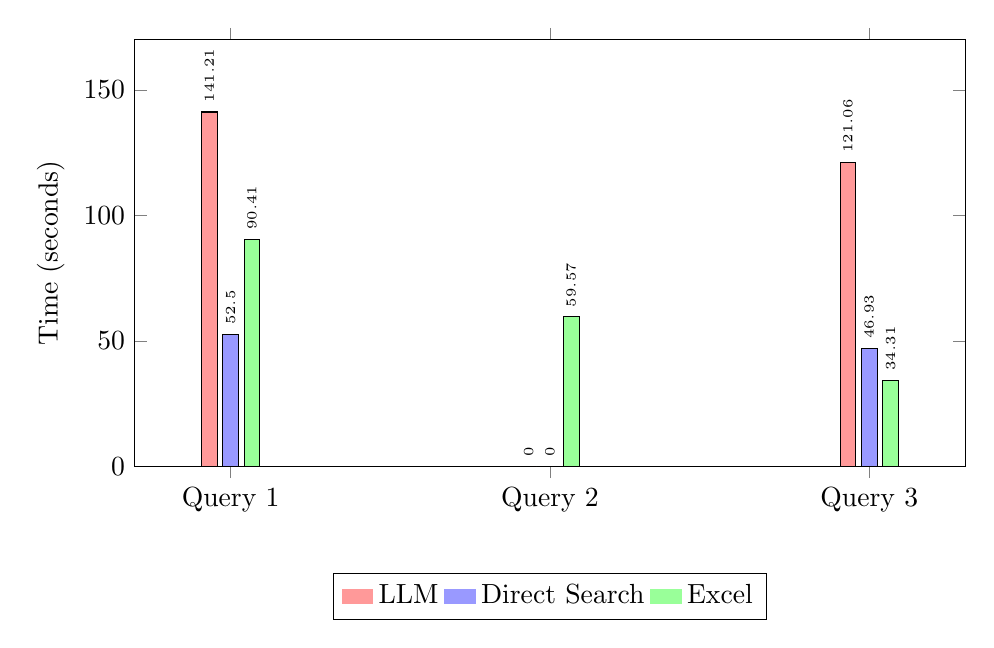
\begin{tikzpicture}
    \begin{axis}[
        ybar=2pt, % Grouped bars
        bar width=0.2cm,
        width=\linewidth,
        height=7cm,
        ylabel={Time (seconds)},
        symbolic x coords={Query 1, Query 2, Query 3},
        xtick=data,
        ymin=0, ymax=170,
        enlarge x limits=0.15, % Space between bar groups
        legend style={at={(0.5,-0.25)}, anchor=north, legend columns=-1},
        % Force legend to show single rectangle instead of double bars
        legend image code/.code={
            \draw[#1, draw=none, fill=#1] (0cm,-0.1cm) rectangle (0.4cm,0.1cm);
        },
        % Standard number formatting for labels
        nodes near coords,
        every node near coord/.append style={font=\tiny, rotate=90, anchor=west},
    ]
    
    % 1. LLM (Red)
    \addplot[fill=red!40] coordinates {(Query 1, 141.21) (Query 2, 0) (Query 3, 121.06)};
    \addlegendentry{LLM}
    
    % 2. Direct Search (Blue)
    \addplot[fill=blue!40] coordinates {(Query 1, 52.5) (Query 2, 0) (Query 3, 46.93)};
    \addlegendentry{Direct Search}
    
    % 3. Excel (Green)
    \addplot[fill=green!40] coordinates {(Query 1, 90.41) (Query 2, 59.57) (Query 3, 34.31)};
    \addlegendentry{Excel}
\end{axis}
\end{tikzpicture}
\caption{Comparison of Time on Task (seconds) across search modalities.}
\label{fig:time_task}
\end{figure}


The discrepancy between the systems is further illustrated by the semantic reversal phenomenon observed during the trials, where the LLM would return records containing "Susceptible" when the user specifically requested "Resistant." This suggests that while the embedding model is effective for broad retrieval, it struggles with the nuance of negative constraints and binary trait attributes. Furthermore, the Direct Search feature, while technically faster, often buried relevant results, forcing users to scan through rows rather than relying on the system’s ranking. This indicates that while the system offers a technological advantage over spreadsheets, its current usability is hindered by inconsistent retrieval accuracy and a steep learning curve for the LLM interaction pattern.


\subsubsection{System Usability Scale (SUS) Results}
The system achieved an average System Usability Scale (SUS) score of 71.5, placing it within the good range of usability and learnability. Individual scores showed significant variance, ranging from a low of 52.5 to a high of 87.5, which mirrors the mixed results observed during the practical task execution. The higher scores indicate that, when the system functions as intended, it offers a promising and natural alternative to traditional data management tools. However, the lower scores reflect frustration stemming from technical inconsistencies, particularly regarding the system's failure to consistently trigger the database search tool and the subsequent retrieval of imprecise or irrelevant data.


\begin{table}[htbp]
\caption{Individual System Usability Scale (SUS) Scores}
\label{tab:sus_scores}
\centering
\begin{tabular}{c|ccccc|c}
\hline
\textbf{User} & U1 & U2 & U3 & U4 & U5 & \textbf{Mean} \\ \hline
\textbf{Score} & 75.0 & 70.0 & 52.5 & 72.5 & 87.5 & \textbf{71.5} \\ \hline
\end{tabular}
\end{table}


Qualitative feedback provided by the participants reinforces the link between these scores and user trust. While the LLM-driven summarization was praised for its accuracy and lack of hallucinations, users frequently expressed difficulty with interface elements, such as the discoverability of the "Add Column" feature and the rigid layout of the table view. Participants often compared the system unfavorably to Excel, noting that while their current spreadsheet-based workflows have their own UI limitations, they provide a level of control—specifically through granular filtering—that the current search implementation lacks. Consequently, while the system demonstrates clear potential to streamline research tasks, improving search precision and refining the user interface to be more explicit remains critical to closing the gap between this new system and established research habits.

\subsection{Qualitative Discussion}
\subsubsection{Limitations in Logical Reasoning}
A critical observation during the usability trials was the system's struggle with binary state distinctions. In several test queries, the system retrieved records marked as "Susceptible" when the user specifically requested "Resistant." This occurs because the embedding model maps the query and the retrieved documents into the same region of latent space based on topic; "Downy Mildew resistance" and "Downy Mildew susceptibility" are conceptually close because they share the same subject matter. The vector space prioritizes this contextual topic over the specific attribute state, leading to a failure in logical precision.

This issue highlights a fundamental limitation of pure semantic retrieval for structured phenotypic data. While the embedding model captures the broader agricultural concepts effectively, it lacks the explicit logic required to parse negations or specific attribute constraints. Moving forward, a hybrid approach is necessary: the system must utilize a metadata-filtering layer to enforce strict Boolean constraints on specific trait columns (e.g., "Downy Mildew" = "Resistant"). This ensures that semantic search acts as the discovery mechanism, while structured filtering ensures the factual accuracy of the results, preventing the system from conflating contradictory attributes.

\subsubsection{Inconsistent Agentic Tool Usage}
The evaluation revealed significant instability in the agentic behavior of the RAG system, particularly regarding the LLM's reliance on the database search tool. Participants frequently encountered scenarios where the LLM provided conversational responses without querying the database, or failed to invoke the search tool unless explicitly instructed by the user. This was not necessarily a deficiency in the retriever component itself, but a failure in the model's instruction-following capabilities under the implemented prompt strategy. The LLM often defaulted to its general training data rather than prioritizing the provided database context.

Interestingly, this technical failure led to an unintended emergent behavior: participants began "hacking" the system by using force-commands such as "search this in db" or "look at the database for X." This indicates that researchers were forced to learn the system's rigid, opaque constraints rather than the system adapting to natural language. This "command-based learning" is a significant hurdle for usability, as it breaks the premise of a user-friendly natural language interface.

To resolve this, future iterations must refine the prompt engineering or the function-calling layer to ensure that when a user intent matches a search task, the database tool is invoked deterministically. The system should not rely on the LLM's probabilistic instruction-following logic alone. By treating the search tool as a mandatory step rather than an optional suggestion, we can ensure consistent behavior and remove the need for users to learn specific, non-intuitive "hack" phrases to trigger database lookups.

\subsubsection{RAG Versus Spreadsheet Paradigms}
The usability trials highlighted a substantial precision gap between the proposed RAG system and the existing spreadsheet workflow. Researchers expressed higher trust in Microsoft Excel not merely due to habit, but because of the deterministic nature of its results. In Excel, a filter for 'Yellow' returns only 'Yellow'; in the RAG system, semantic similarity might surface 'Orange' as conceptually related. While theoretically smarter, this behavior is counter-productive for breeding selections that require strict trait adherence. The AI was perceived as less reliable because it introduced semantic noise where researchers required categorical certainty.

Furthermore, this distrust is exacerbated when the system occasionally provides inaccurate results. When a search fails in Excel, the user typically attributes it to their own filtering logic and corrects it immediately. When the AI fails, the user loses confidence in the entire system, viewing the intelligent suggestions as untrustworthy. This creates a psychological threshold where the AI must perform significantly better than a spreadsheet to be considered good enough, as the error modes of an AI are perceived as more opaque and difficult to troubleshoot than those of a manual spreadsheet filter.

Rather than positioning the RAG system as a replacement for spreadsheets, the findings suggest that it should be integrated as an enhancement to them. A more successful paradigm would be a co-pilot model, where the natural language interface does not merely return an opaque list of results, but instead suggests or automatically applies filters to the current data view. By bridging the gap between natural language intent and the precision of programmatic filtering, the system could provide the conversational convenience of AI without sacrificing the auditability and control that spreadsheet users currently rely on.

\subsubsection{Interface Feature Discoverability Issues}
Participant interaction with the interface revealed that deviating from established UI/UX mental models created significant friction. A prominent example was the "Add Column" task, where participants struggled to find the functionality because it was housed in a non-standard context menu. Users consistently attempted to map their existing knowledge of Excel's interface—specifically, right-clicking on headers or looking for obvious "Edit" or "Insert" buttons—onto the new system. When these expected patterns were not present, cognitive load increased, leading to task frustration even when the backend functionality was fully capable of performing the request.

This suggests that for domain-specific tools used by researchers, UI discoverability is just as important as the underlying model performance. It is recommended that future iterations incorporate explicit, high-visibility signifiers for all administrative tasks. Functions such as record updates, schema modifications, and column management should not be hidden behind nested context menus or abstract icons. By adopting UI patterns consistent with professional data management software, the system can reduce the learning curve and ensure that the administrative overhead does not overshadow the benefits of the semantic search features.

\subsubsection{Data Coverage and Sparsity}
Finally, the failure cases (Queries 5, 10b, 12, 16, and 20) demonstrated that the effectiveness of a semantic search system is inextricably linked to the underlying data density. In instances where the phenotypic trait data was missing, inconsistently recorded, or described using non-standardized terminology, the system could not retrieve meaningful results. Both the lexical baseline and the vector-based system failed because the information simply did not exist in a queryable format. This reinforces the principle that algorithmic sophistication cannot compensate for poor data quality.

This finding leads to the conclusion that data normalization must be prioritized alongside model tuning. The RAG system’s performance is limited by the "semantic density" of the records; if the data is sparse, the embeddings will be noisy, and the search precision will suffer. Future improvements should focus on building a robust data-cleaning pipeline that standardizes phenotypic trait entries before ingestion. By ensuring that terms are consistent and that critical traits are properly populated, the system can be provided with the clean, structured knowledge base required to maximize the accuracy of the semantic search pipeline.

\section{Conclusion and Recommendations}

\subsection{Conclusion}
This study successfully developed and implemented a retrieval-augmented generation (RAG) system specifically tailored to modernize phenotypic trait analysis within the Cereal Crops Section. By integrating a \textit{potion-mxbai-micro} bi-encoder with a ChromaDB vector store and a FastAPI-based backend, the study established a functional, scalable bridge between natural language queries and the Section's existing phenotypic dataset. While the retrieval pipeline proved effective at handling descriptive agricultural queries, the implementation of autonomous agentic capabilities—specifically the function-calling logic within the Qwen3-0.6B LLM—revealed that while the underlying architecture is technically sound, the reliability of autonomous tool invocation remains a significant hurdle for fully hands-free interaction.

Quantitative evaluation of the system’s retrieval performance demonstrated the clear superiority of the two-stage hybrid search pipeline over traditional lexical methods. The system achieved significant improvements in Precision@k over the BM25 keyword baseline, validating the hypothesis that dense semantic search is better equipped to navigate the semantic gap inherent in agricultural terminology. However, the paradox of lower Mean Average Precision (MAP) scores in certain instances underscored that while semantic search is optimal for exploratory discovery, it is not a complete substitute for keyword matching when querying unique identifiers. This evidence supports the conclusion that agricultural search systems must employ a hybrid strategy, balancing the semantic breadth of embeddings with the pinpoint accuracy of lexical matching.

The usability evaluation highlighted that technological superiority in semantic retrieval does not equate to utility if it sacrifices result exactitude. Achieving an average SUS score of 71.5 indicates a promising tool, but the preference for Excel's 'Filter-Sort-Scan' model proves that researchers value deterministic accuracy over algorithmic intuition. To foster trust, the system must mirror the reliability of manual filters by integrating structured query generation into the semantic pipeline.

In summary, this study provides a validated framework for transitioning from manual, keyword-dependent spreadsheet workflows to automated, semantic-driven data discovery. Although the transition from manual control to AI-assisted retrieval presents significant UI/UX challenges, the core retrieval architecture proves that semantic search is a viable, high-performance solution for the Section’s data accessibility needs. By addressing the identified constraints in both retrieval logic and user interface transparency, this study offers a robust model for integrating modern artificial intelligence into specialized agricultural research environments.
    
\subsection{Recommendations}
A fundamental improvement to the system’s performance lies in transitioning from coarse, record-wide serialization to a granular, semantically aware chunking strategy. Currently, treating entire records as single JSON blobs introduces excessive noise, as irrelevant metadata or missing trait placeholders can dilute the signal-to-noise ratio during embedding. Future iterations should implement custom parsing strategies—akin to the structural analysis used for semi-structured documents—to isolate distinct phenotypic traits. By breaking records into logical, trait-specific segments (e.g., separating biotic stress data from agronomic traits) and removing irrelevant headers or watermarks, the system can ensure that each vector represents a clear, self-contained semantic unit. This structured approach, supported by rigorous data cleaning and normalization prior to vectorization, will significantly reduce false positives and improve retrieval accuracy.

Furthermore, a strategic architectural shift is required to bridge the precision gap: moving toward a filter-then-retrieve execution loop. Instead of using the LLM to search the entire vector space immediately, the system should first interpret the user's natural language request to identify deterministic constraints (e.g., specific trait values). The system should prioritize the programmatic application of these Boolean filters to narrow the dataset to a factually precise subset before any semantic retrieval is performed. This filter-first approach ensures that the results are logically sound and verifiable, providing the auditability researchers require, while allowing the semantic retrieval pipeline to operate only on the relevant, filtered subset.

To ensure long-term viability and portability, future research must prioritize the optimization of the system for resource-constrained, self-hosted environments. While current models demonstrate the feasibility of the RAG approach, their reliance on specific hardware can be a barrier to deployment on the Section's aging infrastructure. Future iterations should explore the integration of highly compressed, state-of-the-art static embeddings and quantized LLMs, which provide a balance between linguistic capability and minimal computational overhead. By leveraging these edge-optimized models, the system can maintain high performance and low latency without requiring expensive GPU clusters or cloud-based dependencies, making the tool more accessible and sustainable for independent research groups.

Ultimately, these refinements—structured chunking, programmatic filtering, and edge-optimized modeling—will shift the system from an experimental, autonomous agent to a robust, user-controllable research tool. By moving toward a Co-pilot model, the system sheds its "black-box" limitations, aligning the AI’s operations with the precise, audit-oriented workflows that plant breeders rely on. These changes will not only improve the system's objective retrieval metrics but, more importantly, will foster the necessary user trust to successfully replace legacy spreadsheet workflows with an integrated, intelligent, and transparent data management framework.
% APPENDICES
\appendices

\section{System Usability Scale (SUS) Questionnaire}
The following 10 items will be used to assess the usability of the system. Participants will rate each item on a scale of 1 (Strongly Disagree) to 5 (Strongly Agree).

\begin{enumerate}
    \item I think that I would like to use this system frequently.
    \item I found the system unnecessarily complex.
    \item I thought the system was easy to use.
    \item I think that I would need the support of a technical person to be able to use this system.
    \item I found the various functions in this system were well integrated.
    \item I thought there was too much inconsistency in this system.
    \item I would imagine that most people would learn to use this system very quickly.
    \item I found the system very cumbersome to use.
    \item I felt very confident using the system.
    \item I needed to learn a lot of things before I could get going with this system.
\end{enumerate}

\section{Evaluation Queries}
Table \ref{tab:queries} lists the 20 queries utilized for evaluating the information retrieval performance of both the hybrid and lexical systems.

\begin{table}[htbp]
\caption{Test Queries for IR Evaluation}
\label{tab:queries}
\centering
\begin{tabular}{ll}
\hline
\textbf{ID} & \textbf{Query} \\ \hline
1 & resistant to calcareous soil \\
2 & resistant to calcerous soil (misspelling) \\
3 & early maturing \\
4 & suitable for early harvest \\
5 & purple anther colors \\
6 & ear length greater than 10 cm \\
7 & high yielding \\
8 & tight husk fitting \\
9 & good in very dry soil \\
10 & resistant to drought \\
11 & can handle saturated or flooded soil \\
12 & tolerant to waterlogging \\
13 & shows resistance to ear rot \\
14 & red cob color \\
15 & white cob color \\
16 & resistant to common diseases \\
17 & BT negative Bagtikan \\
18 & purple silk color \\
19 & plant height between 200 and 250 cm \\
20 & more than 13 rows of grain \\ \hline
\end{tabular}
\end{table}

\section{Detailed Information Retrieval Metrics}
The following table provides the per-query performance for the Hybrid Search pipeline. These values were aggregated to produce the summary metrics discussed in Section 5.

\begin{table}[htbp]
\caption{Detailed Performance Metrics for Hybrid Search}
\label{tab:hybrid_metrics_full}
\centering
\resizebox{\columnwidth}{!}{
\begin{tabular}{l|ccc|ccc|c}
\hline
\textbf{Query} & \textbf{P@5} & \textbf{P@10} & \textbf{P@20} & \textbf{R@5} & \textbf{R@10} & \textbf{R@20} & \textbf{MAP} \\ \hline
Query 1 & 0.8 & 0.8 & 0.85 & 0.0186 & 0.0372 & 0.0791 & 0.0652 \\
Query 2 & 1.0 & 0.8 & 0.9 & 0.0233 & 0.0372 & 0.0837 & 0.0757 \\
Query 3 & 1.0 & 0.6 & 0.3 & 0.4545 & 0.5455 & 0.5455 & 0.5455 \\
Query 4b & 0.2 & 0.1 & 0.05 & 0.0909 & 0.0909 & 0.0909 & 0.0909 \\
Query 5 & 0.0 & 0.0 & 0.0 & 0.0000 & 0.0000 & 0.0000 & 0.0000 \\
Query 6 & 0.4 & 0.7 & 0.75 & 0.0250 & 0.0875 & 0.1875 & 0.1259 \\
Query 7 & 0.4 & 0.5 & 0.3 & 0.0606 & 0.1515 & 0.1818 & 0.0896 \\
Query 8 & 0.4 & 0.3 & 0.2 & 0.0400 & 0.0600 & 0.0800 & 0.0532 \\
Query 9 & 0.2 & 0.1 & 0.1 & 0.0045 & 0.0045 & 0.0089 & 0.0050 \\
Query 10b & 0.0 & 0.0 & 0.0 & 0.0000 & 0.0000 & 0.0000 & 0.0000 \\
Query 11 & 0.8 & 0.6 & 0.7 & 0.0179 & 0.0268 & 0.0625 & 0.0466 \\
Query 12 & 0.0 & 0.0 & 0.0 & 0.0000 & 0.0000 & 0.0000 & 0.0000 \\
Query 13 & 0.8 & 0.9 & 0.7 & 0.0101 & 0.0226 & 0.0352 & 0.0302 \\
Query 14 & 0.2 & 0.1 & 0.05 & 0.0164 & 0.0164 & 0.0164 & 0.0033 \\
Query 15 & 0.4 & 0.2 & 0.15 & 0.0500 & 0.0500 & 0.0750 & 0.0233 \\
Query 16 & 0.0 & 0.0 & 0.0 & 0.0000 & 0.0000 & 0.0000 & 0.0000 \\
Query 17 & 1.0 & 1.0 & 0.65 & 0.0169 & 0.0339 & 0.0441 & 0.0438 \\
Query 18 & 0.6 & 0.6 & 0.45 & 0.0349 & 0.0698 & 0.1047 & 0.0690 \\
Query 19 & 0.6 & 0.3 & 0.15 & 1.0000 & 1.0000 & 1.0000 & 1.0000 \\
Query 20 & 0.0 & 0.0 & 0.0 & 0.0000 & 0.0000 & 0.0000 & 0.0000 \\ \hline
\end{tabular}
}
\end{table}

\begin{table}[htbp]
\caption{Detailed Performance Metrics for Keyword Search (BM25)}
\label{tab:keyword_metrics_full}
\centering
\resizebox{\columnwidth}{!}{
\begin{tabular}{l|ccc|ccc|c}
\hline
\textbf{Query} & \textbf{P@5} & \textbf{P@10} & \textbf{P@20} & \textbf{R@5} & \textbf{R@10} & \textbf{R@20} & \textbf{MAP} \\ \hline
Query 1 & 1.0 & 1.0 & 0.85 & 0.0233 & 0.0465 & 0.0791 & 0.0735 \\
Query 2 & 0.0 & 0.0 & 0.00 & 0.0000 & 0.0000 & 0.0000 & 0.0000 \\
Query 3 & 1.0 & 0.7 & 0.35 & 0.4545 & 0.6364 & 0.3500 & 0.6364 \\
Query 4 & 0.0 & 0.0 & 0.00 & 0.0000 & 0.0000 & 0.0000 & 0.0000 \\
Query 5 & 0.0 & 0.0 & 0.00 & 0.0000 & 0.0000 & 0.0000 & 0.0000 \\
Query 6 & 0.0 & 0.0 & 0.00 & 0.0000 & 0.0000 & 0.0000 & 0.0000 \\
Query 7 & 0.2 & 0.5 & 0.30 & 0.0606 & 0.1515 & 0.1818 & 0.0577 \\
Query 8 & 1.0 & 1.0 & 0.90 & 0.1000 & 0.2000 & 0.3600 & 0.3569 \\
Query 9 & 0.0 & 0.0 & 0.00 & 0.0000 & 0.0000 & 0.0000 & 0.0000 \\
Query 10 & 0.0 & 0.0 & 0.00 & 0.0000 & 0.0000 & 0.0000 & 0.0000 \\
Query 11 & 0.8 & 0.8 & 0.80 & 0.0179 & 0.0357 & 0.0714 & 0.0500 \\
Query 12 & 0.0 & 0.0 & 0.00 & 0.0000 & 0.0000 & 0.0000 & 0.0000 \\
Query 13 & 1.0 & 1.0 & 1.00 & 0.0126 & 0.0251 & 0.0503 & 0.0503 \\
Query 14 & 0.2 & 0.1 & 0.05 & 0.0164 & 0.0164 & 0.0164 & 0.0164 \\
Query 15 & 0.0 & 0.0 & 0.00 & 0.0000 & 0.0000 & 0.0000 & 0.0000 \\
Query 16 & 0.0 & 0.0 & 0.00 & 0.0000 & 0.0000 & 0.0000 & 0.0000 \\
Query 17 & 0.2 & 0.1 & 0.05 & 0.0034 & 0.0034 & 0.0034 & 0.0008 \\
Query 18 & 0.0 & 0.0 & 0.00 & 0.0000 & 0.0000 & 0.0000 & 0.0000 \\
Query 19 & 0.6 & 0.3 & 0.15 & 1.0000 & 1.0000 & 1.0000 & 1.0000 \\
Query 20 & 0.2 & 0.2 & 0.10 & 0.2000 & 0.4000 & 0.4000 & 0.2400 \\ \hline
\end{tabular}
}
\end{table}

\section{System Prompt Configuration}
The system utilizes two distinct prompts to manage the interaction loop. The \textit{General Persona Prompt} establishes the constraints for the LLM's natural language generation, while the \textit{Routing Prompt} governs the function-calling logic for database querying.

\subsection{General Persona Prompt}
This prompt is injected into the system message to define the agent's expertise and constraints regarding data synthesis.

\begin{lstlisting}
You are an AI assistant for the Institute of Plant Breeding, specialized in maize phenotypic trait data and parental line selection for plant breeding research. Your primary role is to help the user efficiently query and analyze phenotypic data using natural language, overcoming the limitations of traditional keyword-based searches in spreadsheets. 

Key guidelines:
- Respond in a clear, concise, and helpful manner.
- Ground information in plant breeding principles.
- Do not output markdown or tables.
- If search results are present, do not regurgitate them. Instead, summarize and analyze them.
- Maintain a professional tone suitable for researchers.
\end{lstlisting}

\subsection{Routing and Tool Usage Prompt}
This prompt is used during the intent classification stage to determine the search parameters for the ChromaDB and SQLite backend.

\begin{lstlisting}
You are a search query generator.
Your task is to generate a concise query for the database based on the user's message.
The database contains the following columns: {database_columns}

Your query should be as concise, short, and focused as possible. It should ideally contain only the column to be searched and the search term.

Output ONLY valid JSON: {"query": "search term or none"}
No markdown. No extra text.
\end{lstlisting}

% % ACKNOWLEDGMENT
% \section*{Acknowledgment}
% Many thanks to...

% BIBLIOGRAPHY
\begin{sloppypar}
    \raggedright 
    \bibliographystyle{apacite}
    \bibliography{./glindro-cs190-ieee}
\end{sloppypar}

% BIOGRAPHY
\begin{biography}[{\includegraphics[width=1in, height=1.25in, clip, keepaspectratio]{./glindro.eps}}]{Zach Dwayne M. Glindro}
Biography text here...
\end{biography}


\end{document}